\documentclass[12pt,]{book}
\usepackage{lmodern}
\usepackage{setspace}
\setstretch{1.3}
\usepackage{amssymb,amsmath}
\usepackage{ifxetex,ifluatex}
\usepackage{fixltx2e} % provides \textsubscript
\ifnum 0\ifxetex 1\fi\ifluatex 1\fi=0 % if pdftex
  \usepackage[T1]{fontenc}
  \usepackage[utf8]{inputenc}
\else % if luatex or xelatex
  \ifxetex
    \usepackage{mathspec}
  \else
    \usepackage{fontspec}
  \fi
  \defaultfontfeatures{Ligatures=TeX,Scale=MatchLowercase}
\fi
% use upquote if available, for straight quotes in verbatim environments
\IfFileExists{upquote.sty}{\usepackage{upquote}}{}
% use microtype if available
\IfFileExists{microtype.sty}{%
\usepackage{microtype}
\UseMicrotypeSet[protrusion]{basicmath} % disable protrusion for tt fonts
}{}
\usepackage[left=4cm, right=4cm, top=2.5cm, bottom=2.5cm]{geometry}
\usepackage{hyperref}
\PassOptionsToPackage{usenames,dvipsnames}{color} % color is loaded by hyperref
\hypersetup{unicode=true,
            pdftitle={John's PhD Thesis},
            pdfauthor={John Zobolas},
            colorlinks=true,
            linkcolor=black,
            citecolor=Blue,
            urlcolor=blue,
            breaklinks=true}
\urlstyle{same}  % don't use monospace font for urls
\usepackage{color}
\usepackage{fancyvrb}
\newcommand{\VerbBar}{|}
\newcommand{\VERB}{\Verb[commandchars=\\\{\}]}
\DefineVerbatimEnvironment{Highlighting}{Verbatim}{commandchars=\\\{\}}
% Add ',fontsize=\small' for more characters per line
\usepackage{framed}
\definecolor{shadecolor}{RGB}{248,248,248}
\newenvironment{Shaded}{\begin{snugshade}}{\end{snugshade}}
\newcommand{\AlertTok}[1]{\textcolor[rgb]{0.94,0.16,0.16}{#1}}
\newcommand{\AnnotationTok}[1]{\textcolor[rgb]{0.56,0.35,0.01}{\textbf{\textit{#1}}}}
\newcommand{\AttributeTok}[1]{\textcolor[rgb]{0.77,0.63,0.00}{#1}}
\newcommand{\BaseNTok}[1]{\textcolor[rgb]{0.00,0.00,0.81}{#1}}
\newcommand{\BuiltInTok}[1]{#1}
\newcommand{\CharTok}[1]{\textcolor[rgb]{0.31,0.60,0.02}{#1}}
\newcommand{\CommentTok}[1]{\textcolor[rgb]{0.56,0.35,0.01}{\textit{#1}}}
\newcommand{\CommentVarTok}[1]{\textcolor[rgb]{0.56,0.35,0.01}{\textbf{\textit{#1}}}}
\newcommand{\ConstantTok}[1]{\textcolor[rgb]{0.00,0.00,0.00}{#1}}
\newcommand{\ControlFlowTok}[1]{\textcolor[rgb]{0.13,0.29,0.53}{\textbf{#1}}}
\newcommand{\DataTypeTok}[1]{\textcolor[rgb]{0.13,0.29,0.53}{#1}}
\newcommand{\DecValTok}[1]{\textcolor[rgb]{0.00,0.00,0.81}{#1}}
\newcommand{\DocumentationTok}[1]{\textcolor[rgb]{0.56,0.35,0.01}{\textbf{\textit{#1}}}}
\newcommand{\ErrorTok}[1]{\textcolor[rgb]{0.64,0.00,0.00}{\textbf{#1}}}
\newcommand{\ExtensionTok}[1]{#1}
\newcommand{\FloatTok}[1]{\textcolor[rgb]{0.00,0.00,0.81}{#1}}
\newcommand{\FunctionTok}[1]{\textcolor[rgb]{0.00,0.00,0.00}{#1}}
\newcommand{\ImportTok}[1]{#1}
\newcommand{\InformationTok}[1]{\textcolor[rgb]{0.56,0.35,0.01}{\textbf{\textit{#1}}}}
\newcommand{\KeywordTok}[1]{\textcolor[rgb]{0.13,0.29,0.53}{\textbf{#1}}}
\newcommand{\NormalTok}[1]{#1}
\newcommand{\OperatorTok}[1]{\textcolor[rgb]{0.81,0.36,0.00}{\textbf{#1}}}
\newcommand{\OtherTok}[1]{\textcolor[rgb]{0.56,0.35,0.01}{#1}}
\newcommand{\PreprocessorTok}[1]{\textcolor[rgb]{0.56,0.35,0.01}{\textit{#1}}}
\newcommand{\RegionMarkerTok}[1]{#1}
\newcommand{\SpecialCharTok}[1]{\textcolor[rgb]{0.00,0.00,0.00}{#1}}
\newcommand{\SpecialStringTok}[1]{\textcolor[rgb]{0.31,0.60,0.02}{#1}}
\newcommand{\StringTok}[1]{\textcolor[rgb]{0.31,0.60,0.02}{#1}}
\newcommand{\VariableTok}[1]{\textcolor[rgb]{0.00,0.00,0.00}{#1}}
\newcommand{\VerbatimStringTok}[1]{\textcolor[rgb]{0.31,0.60,0.02}{#1}}
\newcommand{\WarningTok}[1]{\textcolor[rgb]{0.56,0.35,0.01}{\textbf{\textit{#1}}}}
\usepackage{longtable,booktabs}
\usepackage{graphicx,grffile}
\makeatletter
\def\maxwidth{\ifdim\Gin@nat@width>\linewidth\linewidth\else\Gin@nat@width\fi}
\def\maxheight{\ifdim\Gin@nat@height>\textheight\textheight\else\Gin@nat@height\fi}
\makeatother
% Scale images if necessary, so that they will not overflow the page
% margins by default, and it is still possible to overwrite the defaults
% using explicit options in \includegraphics[width, height, ...]{}
\setkeys{Gin}{width=\maxwidth,height=\maxheight,keepaspectratio}
\IfFileExists{parskip.sty}{%
\usepackage{parskip}
}{% else
\setlength{\parindent}{0pt}
\setlength{\parskip}{6pt plus 2pt minus 1pt}
}
\setlength{\emergencystretch}{3em}  % prevent overfull lines
\providecommand{\tightlist}{%
  \setlength{\itemsep}{0pt}\setlength{\parskip}{0pt}}
\setcounter{secnumdepth}{5}
% Redefines (sub)paragraphs to behave more like sections
\ifx\paragraph\undefined\else
\let\oldparagraph\paragraph
\renewcommand{\paragraph}[1]{\oldparagraph{#1}\mbox{}}
\fi
\ifx\subparagraph\undefined\else
\let\oldsubparagraph\subparagraph
\renewcommand{\subparagraph}[1]{\oldsubparagraph{#1}\mbox{}}
\fi

%%% Use protect on footnotes to avoid problems with footnotes in titles
\let\rmarkdownfootnote\footnote%
\def\footnote{\protect\rmarkdownfootnote}

%%% Change title format to be more compact
\usepackage{titling}

% Create subtitle command for use in maketitle
\providecommand{\subtitle}[1]{
  \posttitle{
    \begin{center}\large#1\end{center}
    }
}

\setlength{\droptitle}{-2em}

  \title{John's PhD Thesis}
    \pretitle{\vspace{\droptitle}\centering\huge}
  \posttitle{\par}
  \subtitle{A subtitle of software implementations}
  \author{John Zobolas}
    \preauthor{\centering\large\emph}
  \postauthor{\par}
      \predate{\centering\large\emph}
  \postdate{\par}
    \date{2019-08-07}


\usepackage{amsthm}
\newtheorem{theorem}{Theorem}[chapter]
\newtheorem{lemma}{Lemma}[chapter]
\newtheorem{corollary}{Corollary}[chapter]
\newtheorem{proposition}{Proposition}[chapter]
\newtheorem{conjecture}{Conjecture}[chapter]
\theoremstyle{definition}
\newtheorem{definition}{Definition}[chapter]
\theoremstyle{definition}
\newtheorem{example}{Example}[chapter]
\theoremstyle{definition}
\newtheorem{exercise}{Exercise}[chapter]
\theoremstyle{remark}
\newtheorem*{remark}{Remark}
\newtheorem*{solution}{Solution}
\let\BeginKnitrBlock\begin \let\EndKnitrBlock\end
\begin{document}
\maketitle

{
\hypersetup{linkcolor=black}
\setcounter{tocdepth}{1}
\tableofcontents
}
\listoftables
\listoffigures
\hypertarget{preface}{%
\chapter{Preface}\label{preface}}

What is this thesis about?

\hypertarget{introduction}{%
\section{Introduction}\label{introduction}}

How man became interested in modeling\ldots{}

\hypertarget{phd-work-finished}{%
\chapter{PhD work finished}\label{phd-work-finished}}

Just a summary of all the work (the ``real'' results - investigations/``secondary''
things are not included - that I have achieved in my PhD until now (to write
in bookdown soon).

\hypertarget{pipeline}{%
\section{Pipeline}\label{pipeline}}

\begin{itemize}
\tightlist
\item
  First refactoring, bug fixing, source code documentation on Gitsbe, Drabme,
  druglogics2 (druglogics-synergy) modules and most important parallel simulations
  enabled (my first 2-3 months of my PhD)
\item
  Second refactoring, transport modules to maven packaging, added support
  for many features (Ongoing work - see \href{https://docs.google.com/document/d/1OUupR0b-28YB9pVAww77RMecnFN6A39MYjXMjljmvG4/edit?usp=sharing}{dev\_plan\_doc}).
  Most important things achieved:

  \begin{itemize}
  \tightlist
  \item
    Added tests to modules Gitsbe, Drabme usign JUnit5, mockito, assertJ libraries
  \item
    \href{https://github.com/bblodfon/druglogics-roc-generator}{druglogics-roc-generator}
    R shiny app
  \item
    Export support using \href{https://github.com/colomoto/bioLQM}{BioLQM}: the
    initial model + best generation models can now be exported through configuration
    options to GINML, SBML-Qual and BoolNet community formats
  \end{itemize}
\end{itemize}

\hypertarget{vsm}{%
\section{VSM}\label{vsm}}

\begin{itemize}
\tightlist
\item
  \href{https://github.com/vsmjs/vsm-dictionary-bioportal/}{VSM Dictionary Bioportal} module
\end{itemize}

\hypertarget{psicquic}{%
\section{PSICQUIC}\label{psicquic}}

\begin{itemize}
\tightlist
\item
  miTab 2.8 support added to psicquic web service

  \begin{itemize}
  \tightlist
  \item
    See \href{http://psicquic.github.io/MITAB28Format.html}{psicquic doc here}
  \item
    \href{https://doi.org/10.1093/bioinformatics/btz132}{miTab 2.8/causalTab paper}
  \end{itemize}
\item
  Update \href{https://github.com/MICommunity/psi-jami}{JAMI} library to support
  miTab 2.8 - results of the \href{http://bh2018paris.info/}{BioHackathon 2018, Paris}
  and the \href{https://github.com/GREEKC/hackathon-marseille/tree/master/project_descriptions/causal_psicquic}{Marseille GREEKC hackathon event}.
\end{itemize}

\hypertarget{others}{%
\section{Others}\label{others}}

\begin{itemize}
\tightlist
\item
  Java Client for RSAT tool \href{https://github.com/bblodfon/rsat-rest-java-clients}{fetch-sequences}
\end{itemize}

\hypertarget{phd-plans}{%
\chapter{PhD Plans}\label{phd-plans}}

Plans are currently in terms of technologies. This will change.\footnote{Perhaps}

\hypertarget{pipeline-1}{%
\section{Pipeline}\label{pipeline-1}}

\begin{itemize}
\tightlist
\item
  Ensemble Model biomarker analysis (part of this work is for automated pipeline
  paper). Roadmap:

  \begin{itemize}
  \tightlist
  \item
    Make R package with general useful functions
  \item
    Make R package for biomarker analysis
  \item
    Make bookdown document for previous atopo-based analysis
  \item
    Redo the analysis on Cascade topology and for specific drug combinations (2)
  \item
    Feature importance/biomarker selection using ML methods (compare with what
    you got with your own method, submit to the ML course to get the credits)
  \item
    Submit R packages to CRAN
  \item
    Small publication of the R package and ML methods perhaps?
  \end{itemize}
\item
  Work on the pipeline modules (see the \href{https://docs.google.com/document/d/1OUupR0b-28YB9pVAww77RMecnFN6A39MYjXMjljmvG4/edit?usp=sharing}{dev\_plan\_doc}). Most important:

  \begin{itemize}
  \tightlist
  \item
    Full Testing (Junit 5)
  \item
    BioLQM support: stable state calculation, trap spaces
  \item
    Do comparison between Aurelien's BioLQM stable state algorithm and
    BNReduction using M2
  \end{itemize}
\end{itemize}

\hypertarget{vsm-1}{%
\section{VSM}\label{vsm-1}}

\begin{itemize}
\tightlist
\item
  Make ontologies for genes and proteins known databases (Ensembl, Uniprot)
\item
  PubDictionaries
\item
  Dictionary Merger/Combiner
\end{itemize}

\hypertarget{psicquic-1}{%
\section{PSICQUIC}\label{psicquic-1}}

\begin{itemize}
\tightlist
\item
  Connect data taken from psicquic to atopo (enxtend atopo module to be
  PSICQUIC-compatible - takes causality information and builds network of
  interactions with available configuration on how to do so).
\item
  Help build \href{https://github.com/elixir-europe/BioHackathon/tree/master/interoperability/Prototyping\%20the\%20new\%20PSICQUIC\%202-0}{PSICQUIC 2.0}
\end{itemize}

\hypertarget{synergy}{%
\section{Synergy}\label{synergy}}

\begin{itemize}
\tightlist
\item
  Augment existing R package for calculating reference models to include Wim's
  generalized Bliss method and the mean synergy score by Simone Laderer! Goal
  is to test all the null reference models (Loewe, Bliss, ZIP, +2 new, others?)
  on read dose-response matrix datasets and see which is best at finding the
  synergies. R package to use:

  \begin{itemize}
  \tightlist
  \item
    SynergyFinder from Finland group \href{https://github.com/google/synergyfinderengineered/}{code here}
  \item
    Also see this software: \href{https://www.ncbi.nlm.nih.gov/pmc/articles/PMC5732778/}{R package COMBIA}
  \end{itemize}
\item
  Mathematical formulation of the volume-based synergy score general method to
  include (mine)?
\end{itemize}

\hypertarget{part-miscellaneous-stuff}{%
\part*{Miscellaneous Stuff}\label{part-miscellaneous-stuff}}
\addcontentsline{toc}{part}{Miscellaneous Stuff}

\hypertarget{phd-ideas}{%
\chapter{PhD ideas}\label{phd-ideas}}

\hypertarget{compare-fixpoint-tools}{%
\section{Compare fixpoint tools}\label{compare-fixpoint-tools}}

Compare different tools that calculate fixpoints for logical modeling.

Models used for testing could be of different types:

\begin{itemize}
\tightlist
\item
  self-contained
\item
  varying the number of input nodes (1-n)
\item
  small to large number of nodes
\item
  small to large number of edges
\item
  scale-free (boolnet generated) vs random (varying K connectivity)
\item
  play with form of the boolean equations
\item
  others ???
\end{itemize}

Other things that can be done:

\begin{itemize}
\tightlist
\item
  support BNReduction data format by \href{https://doi.org/10.1186/1471-2105-15-221}{Veliz-Cuba}
  in BioLQM
\item
  add support for calculating the fixpoints using the Colomoto docker (python
  interface)
\item
  comparison between \textbf{BioLQM, Pint, MABOSS and BNReduction} could be done then
  in a Jupiter colomoto-enabled notebook!
\end{itemize}

Further extension/comparisons could be:

\begin{itemize}
\tightlist
\item
  Tamura, 2009 - Integer programming method
\item
  Dubrova, 2009 - SAT-based
\end{itemize}

\hypertarget{use-logical-modeling-to-predict-single-drug-data}{%
\section{Use Logical modeling to predict single-drug data}\label{use-logical-modeling-to-predict-single-drug-data}}

Asmund project proposal: mechanistic drug response prediction analysis

\begin{itemize}
\tightlist
\item
  Automate drug target profile annotation from:

  \begin{itemize}
  \tightlist
  \item
    Klaeger publication 2017 Science
  \item
    mrc ppu
  \item
    Davis publication 2011 (nature biotechnology?)
  \end{itemize}
\item
  Omics data (rna, cnv etc)

  \begin{itemize}
  \tightlist
  \item
    COSMIC
  \item
    CCLE
  \end{itemize}
\item
  Drug scren data

  \begin{itemize}
  \tightlist
  \item
    Single drug

    \begin{itemize}
    \tightlist
    \item
      COSMIC/GDSC
    \item
      CCLE
    \end{itemize}
  \item
    Combo

    \begin{itemize}
    \tightlist
    \item
      O'Neil 2016 Molecular cancer therapeutics
    \item
      FDA Holbeck 2017 cancer research publication
    \end{itemize}
  \end{itemize}
\end{itemize}

\textbf{My idea} is more like this:\\
Predict drug-response curves from drug combination datasets (GDSC, CCLE),
using logical modeling for singaling network analysis or translation from
logical to ODE modeling. Aslo try to predict drug combinations datasets
(dose-response matrices?). Pretty much what is done in this \href{https://doi.org/10.1016/j.cels.2018.10.013}{paper} with help from \href{https://doi.org/10.1186/1752-0509-3-98}{this one}
for converting boolean models to continuous.

\hypertarget{quantum-logic-formalism}{%
\section{Quantum logic formalism}\label{quantum-logic-formalism}}

Instead of logical modeling formalism, use the idea of (queantum) logical gates.
The \textbf{core idea} makes sense: you don't know the state of a protein, but when
you measure it, only then you really know what it is.\\
May also be worth to look at a \href{https://doi.org/10.1007/11885191_18}{game-theoritic approach}
to find attractors and such.

\hypertarget{harmony-search}{%
\section{Harmony Search}\label{harmony-search}}

Use \href{https://doi.org/10.1016/j.proeng.2016.07.510}{this algorithm} for
optimizing the boolean equations for gitsbe?

\hypertarget{druglogics-pipeline-related}{%
\section{Druglogics-Pipeline related}\label{druglogics-pipeline-related}}

\hypertarget{train-models-to-cell-specific-proliferation}{%
\subsection{Train models to cell-specific proliferation}\label{train-models-to-cell-specific-proliferation}}

Concept is that random models predict a lot better than cell-specific ones:
main directive is \textbf{proliferation}, not just fitting to a steady state pattern.

\hypertarget{a-bottom-up-model-building-for-drug-prediction}{%
\subsection{A bottom-up model building for drug prediction}\label{a-bottom-up-model-building-for-drug-prediction}}

Start with a model and some observed synergies. Build/train/produce models that
predict the first observed synergy (using Harmony Search?), from them the next
one, etc. You end up with many models that can predict all the observed
synergies or you try to find out why that cannot happen for example (e.g.~
contrasting synergies?). Do the latest models' stable states or attractors
correspond to activity of proteins from literature?

\hypertarget{simulate-cancer-resistance}{%
\subsection{Simulate cancer resistance}\label{simulate-cancer-resistance}}

For example, you have some models that predict some (observed) synergies or you
just find some synergistic drug comibnations for these models or per model.
Then, you modify these models in order to be resistant to these drugs, simulating
thus the cancer rewiring process! Then, you apply (n+1) drug combinations to
win over the resistance (and you do this procedure at more levels to suggest
3-way, 4-way drug combos and why there might be cancer models that can `win'
over these models and continue the proliferation). You end up with super cancer
resistant models and methods to achieve them or reasons why this cannot happen
at all.

\hypertarget{appendix-appendix}{%
\appendix}


\hypertarget{bookdown-features}{%
\chapter{Bookdown features}\label{bookdown-features}}

Testing stuff!\\
Nice \href{https://eddjberry.netlify.com/post/writing-your-thesis-with-bookdown/}{link}
for reference on how to write a thesis with bookdown.

\hypertarget{references}{%
\section{References}\label{references}}

\begin{itemize}
\tightlist
\item
  Important to remember: Label can be: fig:foo, thm:foo
\item
  Appendix won't have references (figures, tables, equations ain't gonna be
  there)
\item
  Examples

  \begin{itemize}
  \tightlist
  \item
    \protect\hyperlink{vsm-1}{VSM}, \protect\hyperlink{compare-fixpoint-tools}{Compare fixpoint tools}
  \item
    \protect\hyperlink{pipeline-1}{A link to Pipeline}
  \item
    \protect\hyperlink{tables}{Table stuff}
  \item
    A paper citation: Albert et al. (\protect\hyperlink{ref-Albert2008}{2008})
  \item
    Same paper citation: (Albert et al. \protect\hyperlink{ref-Albert2008}{2008})
  \end{itemize}
\end{itemize}

\hypertarget{markdown-examples}{%
\section{Markdown examples}\label{markdown-examples}}

An epigram:

\begin{quote}
``I thoroughly disapprove of duels. If a man should challenge me,
I would take him kindly and forgivingly by the hand and lead him
to a quiet place and kill him.''

--- Mark Twain
\end{quote}

\(f = a\)

\begin{equation} 
  f=a
  \label{eq:binom}
\end{equation}

See Equation \eqref{eq:binom}.

\BeginKnitrBlock{theorem}[Pythagorean theorem]
\protect\hypertarget{thm:pyth}{}{\label{thm:pyth} \iffalse (Pythagorean theorem) \fi{} }For a right triangle, if \(c\) denotes the length of the hypotenuse
and \(a\) and \(b\) denote the lengths of the other two sides, we have
\[a^2 + b^2 = c^2\]
\EndKnitrBlock{theorem}

See Theorem \ref{thm:pyth}.

\BeginKnitrBlock{definition}[Pythagorean theorem]
\protect\hypertarget{def:pyth-def}{}{\label{def:pyth-def} \iffalse (Pythagorean theorem) \fi{} }For a right triangle, if \(c\) denotes the length of the hypotenuse
and \(a\) and \(b\) denote the lengths of the other two sides, we have
\[a^2 + b^2 = c^2\]
\EndKnitrBlock{definition}

See Definition \ref{def:pyth-def}.

\hypertarget{figures}{%
\section{Figures}\label{figures}}

A normal paragraph.



\begin{figure}
\centering
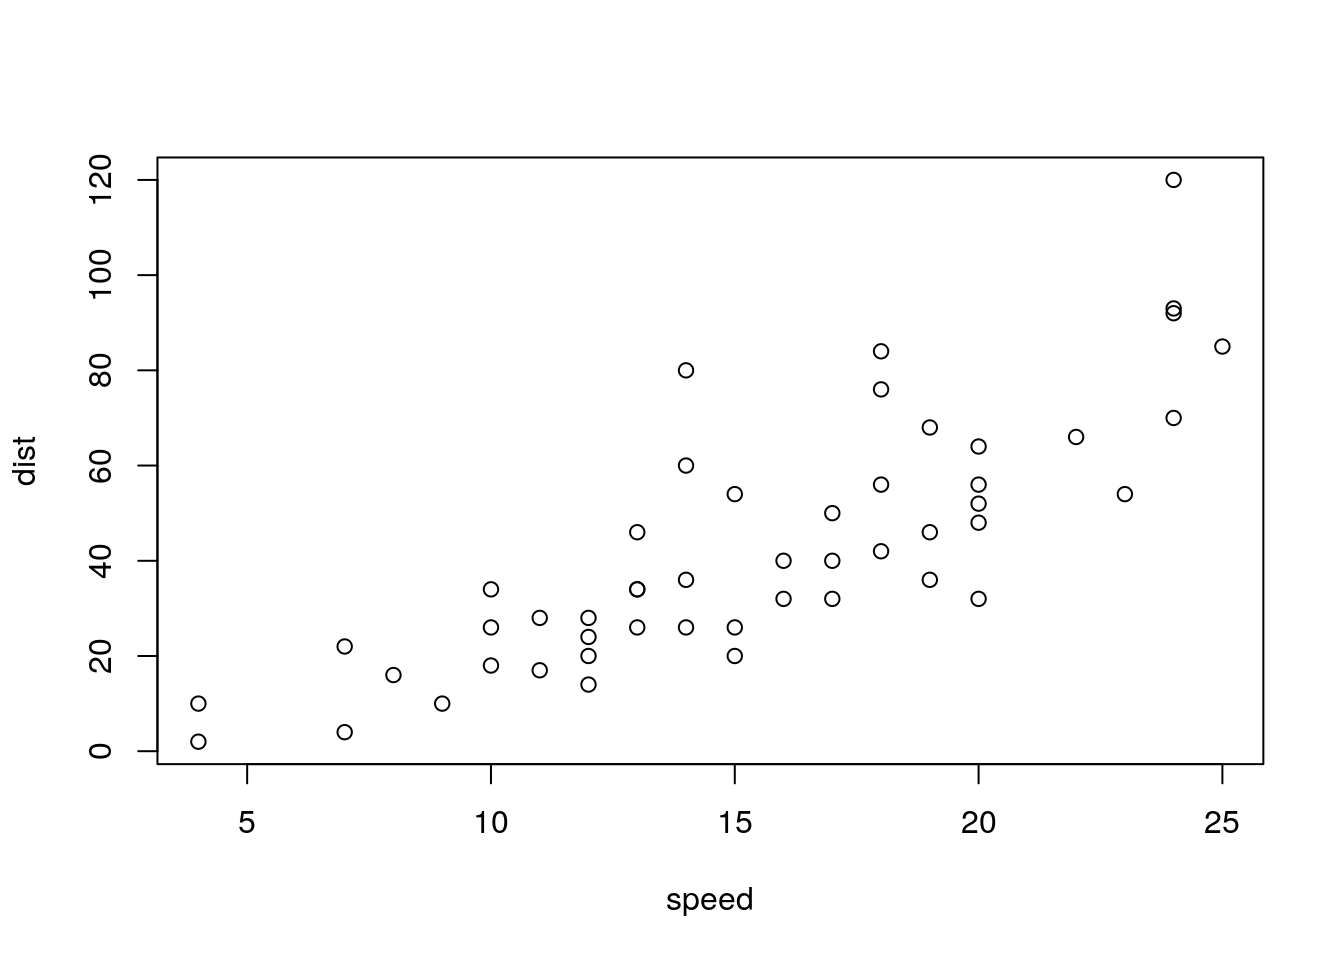
\includegraphics{phd-thesis_files/figure-latex/foo-1.pdf}
\caption{\label{fig:foo}A scatterplot of the data \texttt{cars} using \textbf{base} R graphics.}
\end{figure}

\begin{figure}

{\centering 
\includegraphics[width=0.45\linewidth]{img/questions} 

}

\caption{A Big Question}\label{fig:question}
\end{figure}

See Figure \ref{fig:question}!

\hypertarget{tables}{%
\section{Tables}\label{tables}}

\begin{table}[t]

\caption{\label{tab:table1}A table of the first 5 rows of the mtcars data.}
\centering
\begin{tabular}{lrrrrrrrr}
\toprule
  & mpg & cyl & disp & hp & drat & wt & qsec & vs\\
\midrule
Mazda RX4 & 21.0 & 6 & 160 & 110 & 3.90 & 2.620 & 16.46 & 0\\
Mazda RX4 Wag & 21.0 & 6 & 160 & 110 & 3.90 & 2.875 & 17.02 & 0\\
Datsun 710 & 22.8 & 4 & 108 & 93 & 3.85 & 2.320 & 18.61 & 1\\
Hornet 4 Drive & 21.4 & 6 & 258 & 110 & 3.08 & 3.215 & 19.44 & 1\\
Hornet Sportabout & 18.7 & 8 & 360 & 175 & 3.15 & 3.440 & 17.02 & 0\\
\bottomrule
\end{tabular}
\end{table}

See Table \ref{tab:table1}

\begin{Shaded}
\begin{Highlighting}[]
\NormalTok{DT}\OperatorTok{::}\KeywordTok{datatable}\NormalTok{(iris)}
\end{Highlighting}
\end{Shaded}

\includegraphics{phd-thesis_files/figure-latex/exam-1.pdf}

\hypertarget{another-appendix}{%
\chapter{Another appendix!!!}\label{another-appendix}}

Software used, inspirations, etc.

\hypertarget{references-1}{%
\chapter*{References}\label{references-1}}
\addcontentsline{toc}{chapter}{References}

\hypertarget{refs}{}
\leavevmode\hypertarget{ref-Albert2008}{}%
Albert, István, Juilee Thakar, Song Li, Ranran Zhang, and Réka Albert. 2008. ``Boolean network simulations for life scientists.'' \emph{Source Code for Biology and Medicine} 3: 16. \url{https://doi.org/10.1186/1751-0473-3-16}.


\end{document}
